% SC4022 --- Chapter 1: Network Foundations & Graph Models (0->100 ground-up)
\chapter{Network Foundations \& Graph Models}
\label{ch:foundations}
\sloppy

\begin{quote}
\emph{``A network is more than its parts.''} --- From a handful of friends to the entire Web, the pattern of connections shapes what the whole system can do. Before measuring importance or modelling growth, we need a language for that pattern.
\end{quote}

\noindent\fbox{\parbox{\dimexpr\linewidth-2\fboxsep-2\fboxrule}{%
\textbf{From zero: we build here, no prior graph theory needed.} We assume only sets and basic counting. Every notion---node, edge, degree, path, component---is motivated by a picture, then defined, then exercised. No prior bachelor's knowledge is required.}}
\vspace{0.4em}

\section*{Learning Outcomes}
After this chapter you will be able to:
\begin{enumerate}[label=(L\arabic*)]
    \item define graphs, directed, weighted and bipartite variants and their adjacency representations;
    \item compute degree, degree distribution, and handshaking properties on small examples;
    \item explain paths, components, diameter, and clustering coefficient intuitively and formally;
    \item classify canonical models: lattice, tree, complete, star, bipartite, and their trade-offs;
    \item build and manipulate graphs in Python (NetworkX) choosing list vs matrix.
\end{enumerate}

% ============================================================
\section{What Is a Network?}
\label{sec:what-is-network}
\paragraph{Intuition.} Picture four people: Alice knows Bob and Carol; Bob knows Carol and Dave. Draw a dot for each person, a line for each acquaintance. The dots-and-lines picture \emph{is} the network. The dots are ``where things are''; the lines are ``what connects to what.'' That is all a network is---yet from this spare picture we can ask rich questions: who is most connected? how far does news travel? does the network split into islands?

\paragraph{Formal view.} A \emph{graph} $G=(V,E)$ is a finite set $V$ of \emph{nodes} (vertices) and a set $E$ of \emph{edges} linking them. For undirected graphs an edge is an unordered pair $\{u,v\}$ with $u\neq v$ (no self-loops for now). We write $n=|V|$, $m=|E|$. Variants add direction or weight.

\begin{definition}[Graph and variants]\label{def:graph}
An \emph{undirected simple graph} is $G=(V,E)$ with $E\subseteq\binom{V}{2}$. A \emph{directed graph} has $E\subseteq V\times V$ (ordered pairs, arrows). A \emph{weighted graph} adds $w:E\to\mathbb{R}$ (e.g.\ distance, strength). A \emph{bipartite graph} has $V=V_1\cup V_2$, $V_1\cap V_2=\emptyset$, and every edge joins $V_1$ to $V_2$. A \emph{multigraph} allows multiple edges; a \emph{self-loop} is $\{v,v\}$.
\end{definition}

\begin{figure}[h]\centering
\begin{tikzpicture}[scale=0.78,every node/.style={font=\scriptsize}]
\begin{scope}
\node[font=\footnotesize\bfseries] at (1.35,2.6) {Undirected};
\node[circle,draw,thick,fill=blue!15,minimum size=0.65cm] (a1) at (0,1.5) {A};
\node[circle,draw,thick,fill=blue!15,minimum size=0.65cm] (b1) at (2.7,1.5) {B};
\node[circle,draw,thick,fill=blue!15,minimum size=0.65cm] (c1) at (0,0) {C};
\node[circle,draw,thick,fill=blue!15,minimum size=0.65cm] (d1) at (2.7,0) {D};
\draw[thick] (a1)--(b1); \draw[thick] (b1)--(d1); \draw[thick] (a1)--(c1); \draw[thick] (c1)--(d1);
\node[font=\tiny,fill=blue!8,rounded corners=2pt,inner sep=2pt] at (1.35,-0.7) {$E=\{\{A,B\},\dots\}$};
\end{scope}
\begin{scope}[xshift=4.2cm]
\node[font=\footnotesize\bfseries] at (1.35,2.6) {Directed};
\node[circle,draw,thick,fill=green!15,minimum size=0.65cm] (a2) at (0,1.5) {A};
\node[circle,draw,thick,fill=green!15,minimum size=0.65cm] (b2) at (2.7,1.5) {B};
\node[circle,draw,thick,fill=green!15,minimum size=0.65cm] (c2) at (0,0) {C};
\node[circle,draw,thick,fill=green!15,minimum size=0.65cm] (d2) at (2.7,0) {D};
\draw[->,thick,>=Stealth] (a2) to (b2); \draw[->,thick,>=Stealth] (b2) to (d2); \draw[->,thick,>=Stealth] (c2) to (a2);
\node[font=\tiny,fill=green!8,rounded corners=2pt,inner sep=2pt] at (1.35,-0.7) {arrows: $(A,B)\neq(B,A)$};
\end{scope}
\begin{scope}[xshift=8.4cm]
\node[font=\footnotesize\bfseries] at (1.35,2.6) {Weighted};
\node[circle,draw,thick,fill=orange!15,minimum size=0.65cm] (a3) at (0,1.5) {A};
\node[circle,draw,thick,fill=orange!15,minimum size=0.65cm] (b3) at (2.7,1.5) {B};
\node[circle,draw,thick,fill=orange!15,minimum size=0.65cm] (c3) at (0,0) {C};
\node[circle,draw,thick,fill=orange!15,minimum size=0.65cm] (d3) at (2.7,0) {D};
\draw[thick] (a3)--(b3) node[midway,above,font=\tiny,fill=white,inner sep=1pt] {2.1};
\draw[thick] (b3)--(d3) node[midway,right,font=\tiny,fill=white,inner sep=1pt] {0.8};
\draw[thick] (a3)--(c3) node[midway,left,font=\tiny,fill=white,inner sep=1pt] {5.0};
\node[font=\tiny,fill=orange!8,rounded corners=2pt,inner sep=2pt] at (1.35,-0.7) {$w:E\to\mathbb{R}$};
\end{scope}
\begin{scope}[xshift=12.4cm,yshift=0.2cm]
\node[font=\footnotesize\bfseries] at (1.1,2.4) {Bipartite};
\node[circle,draw,thick,fill=violet!14,minimum size=0.6cm] (u1) at (0,1.6) {U1};
\node[circle,draw,thick,fill=violet!14,minimum size=0.6cm] (u2) at (0,0.5) {U2};
\node[circle,draw,thick,fill=yellow!16,minimum size=0.6cm] (v1) at (2.2,1.6) {V1};
\node[circle,draw,thick,fill=yellow!16,minimum size=0.6cm] (v2) at (2.2,0.5) {V2};
\draw[thick,violet!60!black] (u1)--(v1); \draw[thick,violet!60!black] (u1)--(v2); \draw[thick,violet!60!black] (u2)--(v1);
\node[font=\tiny,fill=violet!8,rounded corners=2pt,inner sep=2pt] at (1.1,-0.9) {edges only $U\to V$};
\end{scope}
\node[font=\tiny,draw=gray!40,fill=yellow!8,rounded corners=2pt,inner sep=3pt] at (6.5,-1.55) {\textcolor{blue!60!black}{$\blacksquare$ undirected} \quad \textcolor{green!50!black}{$\blacksquare$ directed} \quad \textcolor{orange!70!black}{$\blacksquare$ weighted} \quad \textcolor{violet!60!black}{$\blacksquare$ bipartite}};
\end{tikzpicture}
\caption{Four graph flavours. Colour distinguishes edge meaning. Undirected edges are symmetric friendships; directed edges are follows or citations; weights encode distance or strength; bipartite edges cross the partition.}
\label{fig:graph-types}
\end{figure}

Two representations compete. The \emph{adjacency matrix} $A$ is $n\times n$ with $A_{ij}=1$ if $\{i,j\}\in E$ (or weight). The \emph{adjacency list} stores for each node its neighbours. Matrix checks ``is there an edge?'' in $O(1)$ but uses $\Theta(n^2)$ memory; list uses $\Theta(n+m)$ and iterates neighbours fast---best for sparse real networks where $m\ll n^2$.

% ============================================================
\section{Degree, Paths, and Components}
\label{sec:degree-paths}
\paragraph{Intuition.} If you count the lines touching a dot, you know how sociable that person is. If you can hop dot-to-dot from $s$ to $t$, they are in the same island; if not, the network is split. The shortest hop-count is a distance.

\begin{definition}[Degree, path, component]\label{def:degree-path}
The \emph{degree} $k_v=|N(v)|$ counts neighbours of $v$. The \emph{degree distribution} $P(k)$ is the fraction of nodes with degree $k$; the \emph{average degree} is $\langle k\rangle=2m/n$. A \emph{path} is a sequence $v_0,v_1,\dots,v_\ell$ with $\{v_{i},v_{i+1}\}\in E$. Its \emph{length} is $\ell$ (edges). The \emph{distance} $d(s,t)$ is the shortest path length (or $\infty$ if disconnected). A \emph{connected component} is a maximal connected subgraph. The \emph{diameter} is $\max_{s,t}d(s,t)$ over the largest component.
\end{definition}

The \emph{handshaking lemma} is a first theorem: $\sum_v k_v=2m$ because each edge contributes one to the degree at each end. Average degree follows immediately. On Fig.~\ref{fig:path-component}, node $3$ has degree $3$ (most connected), nodes $1$ and $8$ have degree $1$.

\begin{figure}[h]\centering
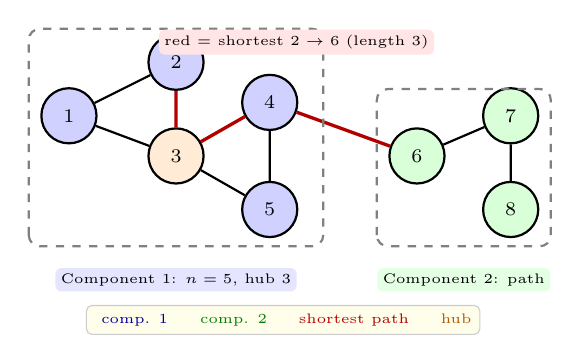
\begin{tikzpicture}[scale=0.85,every node/.style={font=\scriptsize}]
\node[circle,draw,thick,fill=blue!18,minimum size=0.7cm] (1) at (0,1.6) {1};
\node[circle,draw,thick,fill=blue!18,minimum size=0.7cm] (2) at (1.6,2.4) {2};
\node[circle,draw,thick,fill=orange!16,minimum size=0.7cm] (3) at (1.6,1.0) {3};
\node[circle,draw,thick,fill=blue!18,minimum size=0.7cm] (4) at (3.0,1.8) {4};
\node[circle,draw,thick,fill=blue!18,minimum size=0.7cm] (5) at (3.0,0.2) {5};
\node[circle,draw,thick,fill=green!15,minimum size=0.7cm] (6) at (5.2,1.0) {6};
\node[circle,draw,thick,fill=green!15,minimum size=0.7cm] (7) at (6.6,1.6) {7};
\node[circle,draw,thick,fill=green!15,minimum size=0.7cm] (8) at (6.6,0.2) {8};
\draw[thick] (1)--(2); \draw[thick,red!70!black,line width=1.2pt] (2)--(3); \draw[thick,red!70!black,line width=1.2pt] (3)--(4); \draw[thick,red!70!black,line width=1.2pt] (4)--(6);
\draw[thick] (1)--(3); \draw[thick] (3)--(5); \draw[thick] (4)--(5); \draw[thick] (6)--(7); \draw[thick] (7)--(8);
\draw[dashed,gray,thick,rounded corners=4pt] (-0.6,-0.35) rectangle (3.8,2.9);
\draw[dashed,gray,thick,rounded corners=4pt] (4.6,-0.35) rectangle (7.2,2.0);
\node[font=\tiny,fill=blue!10,rounded corners=2pt,inner sep=2pt] at (1.6,-0.85) {Component 1: $n=5$, hub 3};
\node[font=\tiny,fill=green!10,rounded corners=2pt,inner sep=2pt] at (5.9,-0.85) {Component 2: path};
\node[font=\tiny,fill=red!10,rounded corners=2pt,inner sep=2pt] at (3.4,2.7) {red = shortest $2\to6$ (length 3)};
\node[font=\tiny,draw=gray!40,fill=yellow!8,rounded corners=2pt,inner sep=3pt] at (3.2,-1.45) {\textcolor{blue!60!black}{$\blacksquare$ comp. 1} \quad \textcolor{green!50!black}{$\blacksquare$ comp. 2} \quad \textcolor{red!70!black}{$\blacksquare$ shortest path} \quad \textcolor{orange!70!black}{$\blacksquare$ hub}};
\end{tikzpicture}
\caption{Paths and components on an 8-node graph. Two components: $\{1,2,3,4,5\}$ and $\{6,7,8\}$. The shortest path $2\to6$ has length 3 (red). Node 3 is the degree hub. Diameter of the left component is 3.}
\label{fig:path-component}
\end{figure}

\paragraph{Clustering: are my friends friends?} The \emph{clustering coefficient} formalises triangle density. Locally, $C_v=(\text{edges among neighbours of }v)/\binom{k_v}{2}$ (or 0 if $k_v<2$). Globally, $C=(1/n)\sum_v C_v$ or transitivity $3\times\text{triangles}/\text{connected triples}$. A network where ``friends of friends are friends'' has high $C$.

\begin{example}[Small worked clustering]\label{ex:clustering}
In Fig.~\ref{fig:path-component}, neighbours of node 3 are $\{1,2,5\}$. Among them, edges present: $\{1,2\}$ only, so $C_3=1/\binom{3}{2}=1/3$. Node 1 has neighbours $\{2,3\}$ with edge $\{2,3\}$ present, so $C_1=1$. Node 6 has neighbours $\{4,7\}$ with no edge between them, so $C_6=0$. Average $C\approx0.27$ for this graph.
\end{example}

% ============================================================
\section{Canonical Graph Models}
\label{sec:canonical}
\paragraph{Intuition.} Before asking ``what does Facebook look like?'' we describe extremes to calibrate intuition: a ring where everyone knows neighbours (ordered), a tree with no cycles (hierarchical), a clique where everyone knows everyone (dense), and a star centred on one hub (unequal). Real networks sit between these.

\begin{definition}[Canonical models]\label{def:canonical}
A \emph{path} $P_n$ and \emph{cycle} $C_n$ have $n$ nodes in a line or ring. A \emph{complete graph} $K_n$ has all $\binom{n}{2}$ edges ($k_v=n-1$). A \emph{star} $S_n$ has one centre linked to $n-1$ leaves. A \emph{tree} has $n-1$ edges, no cycles. A \emph{regular lattice} links each node to its $k$ nearest neighbours on a ring. A \emph{bipartite complete} $K_{a,b}$ links every $a$ on the left to every $b$ on the right.
\end{definition}

\begin{figure}[h]\centering
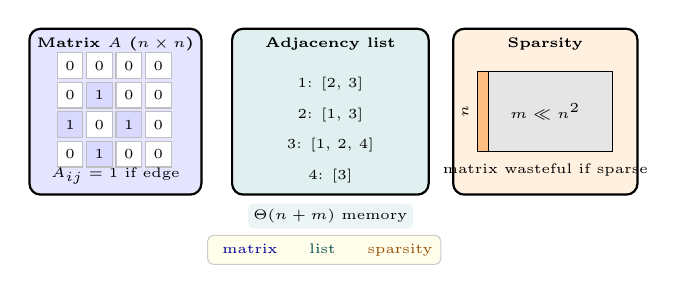
\begin{tikzpicture}[scale=0.78,every node/.style={font=\scriptsize}]
\draw[thick,fill=blue!10,rounded corners=4pt] (-0.3,-0.3) rectangle (2.5,2.4);
\node[font=\tiny\bfseries] at (1.1,2.15) {Matrix $A$ ($n\times n$)};
\foreach \x in {0,...,3} \foreach \y in {0,...,3} {\pgfmathsetmacro{\c}{\x==1&&\y==0 ? 15 : (\x==0&&\y==1 ? 15 : (\x==2&&\y==1 ? 15 : (\x==1&&\y==2 ? 15 : 0)))}
\draw[fill=blue!\c,draw=gray!50] (0.15+0.48*\x,0.15+0.48*\y) rectangle +(0.42,0.42);
\node[font=\tiny] at (0.36+0.48*\x,0.36+0.48*\y) {\pgfmathparse{\c>0 ? 1 : 0}\pgfmathresult};}
\node[font=\tiny] at (1.1,0.0) {$A_{ij}=1$ if edge};
\draw[thick,fill=teal!12,rounded corners=4pt] (3.0,-0.3) rectangle (6.2,2.4);
\node[font=\tiny\bfseries] at (4.6,2.15) {Adjacency list};
\node[font=\tiny,align=left] at (4.6,1.5) {1: [2, 3]};
\node[font=\tiny,align=left] at (4.6,1.0) {2: [1, 3]};
\node[font=\tiny,align=left] at (4.6,0.5) {3: [1, 2, 4]};
\node[font=\tiny,align=left] at (4.6,0.0) {4: [3]};
\node[font=\tiny,fill=teal!8,rounded corners=2pt,inner sep=2pt] at (4.6,-0.65) {$\Theta(n+m)$ memory};
\begin{scope}[xshift=6.8cm]
\draw[thick,fill=orange!12,rounded corners=4pt] (-0.2,-0.3) rectangle (2.8,2.4);
\node[font=\tiny\bfseries] at (1.3,2.15) {Sparsity};
\draw[fill=gray!20] (0.2,0.4) rectangle (2.4,1.7);
\draw[fill=orange!50] (0.2,0.4) rectangle (0.38,1.7);
\node[font=\tiny,rotate=90] at (0.0,1.05) {$n$};
\node[font=\tiny] at (1.3,1.05) {$m\ll n^2$};
\node[font=\tiny] at (1.3,0.1) {matrix wasteful if sparse};
\end{scope}
\node[font=\tiny,draw=gray!40,fill=yellow!8,rounded corners=2pt,inner sep=3pt] at (4.5,-1.2) {\textcolor{blue!60!black}{$\blacksquare$ matrix} \quad \textcolor{teal!60!black}{$\blacksquare$ list} \quad \textcolor{orange!60!black}{$\blacksquare$ sparsity}};
\end{tikzpicture}
\caption{Matrix vs list representation. Matrix is dense $n\times n$ (left); list stores only neighbours (centre). For sparse networks ($m\ll n^2$) the list wins by far (right).}
\label{fig:repr}
\end{figure}

\begin{lstlisting}[language=Python, caption={Building and inspecting graphs with NetworkX: representations and basic measures.}, label={lst:basics}]
import networkx as nx

G = nx.karate_club_graph()          # Zachary karate: 34 nodes, 78 edges
print(f"n={G.number_of_nodes()} m={G.number_of_edges()}"
      f" <k>={2*G.number_of_edges()/G.number_of_nodes():.2f}")

# Degree and distribution
degrees = [d for _, d in G.degree()]
print("max degree:", max(degrees), "min degree:", min(degrees))

# Clustering and diameter (largest component)
print("avg clustering:", round(nx.average_clustering(G), 3))
print("diameter:", nx.diameter(G))

# Adjacency matrix vs list (sparse check)
import numpy as np
A = nx.to_numpy_array(G)            # n x n dense
print("matrix shape:", A.shape, "sparsity:", (A==0).sum()/A.size)
print("list for node 0:", list(G.neighbors(0))[:5])
\end{lstlisting}

\begin{lstlisting}[language=Python, caption={Canonical models: lattice, star, and bipartite gallery.}, label={lst:canonical}]
import matplotlib.pyplot as plt

models = {
    "Cycle C8": nx.cycle_graph(8),
    "Star S7": nx.star_graph(6),
    "Complete K5": nx.complete_graph(5),
    "Tree": nx.balanced_tree(r=2, h=3),
}
for name, H in models.items():
    print(name, f"n={H.number_of_nodes()} m={H.number_of_edges()}"
          f" diam={nx.diameter(H) if nx.is_connected(H) else 'inf'}"
          f" C={nx.average_clustering(H):.2f}")
# Bipartite: 3 producers - 4 consumers
B = nx.complete_bipartite_graph(3, 4)
print("K3,4 edges:", B.number_of_edges(), "is_bipartite:", nx.is_bipartite(B))
\end{lstlisting}

% ============================================================
\section{Chapter Notes}
Real-network thinking begins with Euler (1736) on the K\"onigsberg bridges---nodes and edges abstracting geography. Modern Network Science (Barab\'asi, 2016; Newman, 2018) systematised degree distributions, clustering, and diameter as the three lenses used in this chapter. For sparse-network algorithms, adjacency lists with BFS/DFS remain the workhorse from SC2001; matrix methods dominate spectral analyses (Ch.~3). The Zachary karate club dataset used above will recur throughout this book as a running example.

% ============================================================
\section{Exercises}
\label{sec:ch01-exercises}
\begin{enumerate}[label=E1.\arabic*, leftmargin=*, itemsep=0.8em]
    \item \textbf{Handshake lemma.} A graph has degree sequence $[3,2,2,1,1,1]$. How many edges? Draw one such graph or prove none exists. State and prove $\sum_v k_v=2m$ and deduce $n\langle k\rangle=2m$.
    \item \textbf{Matrix vs list.} For $n=10^5$, $m=5\times10^5$, estimate memory for adjacency matrix (1 byte per entry, symmetric) vs adjacency list (4 bytes per int + overhead). Which fits in 1 GB? At what $m$ does matrix become competitive?
    \item \textbf{Clustering by hand.} On a 5-node house graph (square $1$-$2$-$3$-$4$-$1$ plus roof $2$-$5$-$3$), compute $C_v$ for each $v$ and the average $C$. Compute transitivity and compare. Which node has highest local clustering?
    \item \textbf{Diameter chase.} Find the diameter of: (a) $P_n$, (b) $C_n$, (c) $K_n$, (d) star $S_n$, (e) $K_{2,5}$ (use BFS reasoning, no code). Which grows with $n$ and which stays constant?
    \item \textbf{Build and verify.} Using NetworkX, build a 12-node ring lattice where each node links to its 2 nearest neighbours on each side ($k=4$). Report $m$, average clustering, and diameter. Then rewire 2 random edges and report how each metric changes.
\end{enumerate}
% End of Chapter 1
